\documentclass[border=5pt]{standalone}
\usepackage{tikz}
\usepackage{amsmath}
\usetikzlibrary{arrows.meta,positioning}
\begin{document}
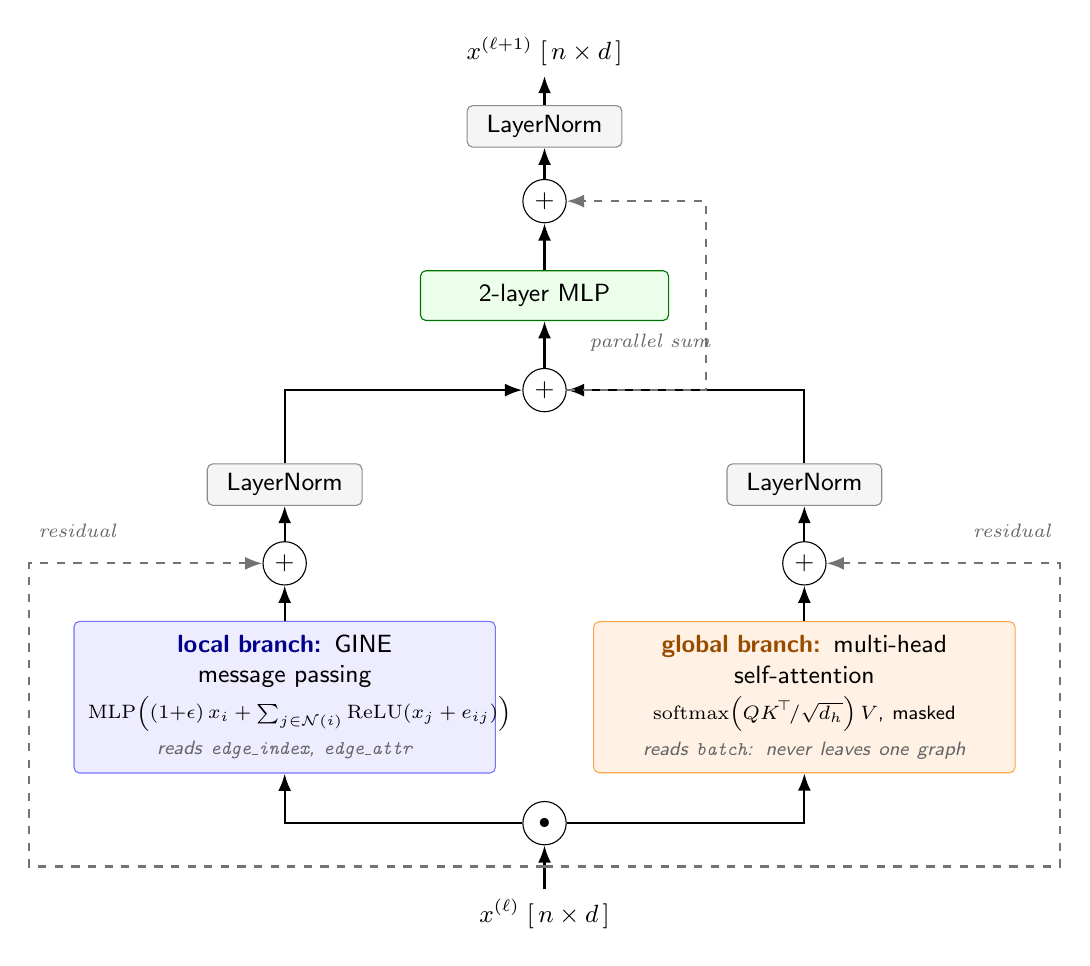
\begin{tikzpicture}[
  x=1cm, y=1cm, font=\sffamily\small,
  box/.style={draw, rounded corners=2pt, align=center, inner sep=5pt},
  norm/.style={draw, rounded corners=2pt, fill=black!4, draw=black!45, inner xsep=7pt, inner ysep=3.5pt},
  op/.style={draw, circle, inner sep=0.5pt, minimum size=5.5mm, fill=white},
  ar/.style={-{Latex[length=2.2mm]}, thick},
  res/.style={-{Latex[length=2.2mm]}, thick, dashed, black!55},
  note/.style={font=\scriptsize\itshape, text=black!60},
]
\def\XL{-3.3} \def\XR{3.3} \def\RL{-6.55} \def\RR{6.55}

% ---- nodes -------------------------------------------------------------
\node (in)   at (0,-0.3) {$x^{(\ell)}\;[\,n\times d\,]$};
\node[op]    (split) at (0,0.85) {\footnotesize$\bullet$};

\node[box, fill=blue!7,   draw=blue!55,      text width=50mm] (mp) at (\XL,2.45)
  {{\bfseries\color{blue!55!black}local branch:} GINE\\ message passing\\[2pt]
   {\scriptsize$\mathrm{MLP}\!\left((1{+}\epsilon)\,x_i+\textstyle\sum_{j\in\mathcal N(i)}\mathrm{ReLU}(x_j+e_{ij})\right)$}\\[2pt]
   {\scriptsize\itshape\color{black!60} reads \texttt{edge\_index}, \texttt{edge\_attr}}};
\node[box, fill=orange!10, draw=orange!70,   text width=50mm] (at) at (\XR,2.45)
  {{\bfseries\color{orange!60!black}global branch:} multi-head\\ self-attention\\[2pt]
   {\scriptsize$\mathrm{softmax}\!\left(QK^{\!\top}\!/\sqrt{d_h}\right)V$, masked}\\[2pt]
   {\scriptsize\itshape\color{black!60} reads \texttt{batch}: never leaves one graph}};

\node[op]   (p1) at (\XL,4.15) {$+$};        \node[op]   (p2) at (\XR,4.15) {$+$};
\node[norm] (n1) at (\XL,5.15) {LayerNorm};  \node[norm] (n2) at (\XR,5.15) {LayerNorm};
\node[op]   (sum) at (0,6.35) {$+$};
\node[box, fill=green!8, draw=green!45!black, text width=28mm] (ffn) at (0,7.55) {2-layer MLP};
\node[op]   (p3) at (0,8.75) {$+$};
\node[norm] (n3) at (0,9.7) {LayerNorm};
\node       (out) at (0,10.65) {$x^{(\ell+1)}\;[\,n\times d\,]$};

% ---- main path ---------------------------------------------------------
\draw[ar] (in) -- (split);
\draw[ar] (split) -- (\XL,0.85) -- (mp);
\draw[ar] (split) -- (\XR,0.85) -- (at);
\draw[ar] (mp) -- (p1);   \draw[ar] (at) -- (p2);
\draw[ar] (p1) -- (n1);   \draw[ar] (p2) -- (n2);
\draw[ar] (n1) -- (\XL,6.35) -- (sum);
\draw[ar] (n2) -- (\XR,6.35) -- (sum);
\draw[ar] (sum) -- (ffn);
\draw[ar] (ffn) -- (p3);
\draw[ar] (p3) -- (n3);
\draw[ar] (n3) -- (out);

% ---- residual connections ---------------------------------------------
\draw[res] (0,0.3) -- (\RL,0.3) -- (\RL,4.15) -- (p1);
\draw[res] (0,0.3) -- (\RR,0.3) -- (\RR,4.15) -- (p2);
\draw[res] (sum)   -- (2.05,6.35) -- (2.05,8.75) -- (p3);

\node[note, anchor=south west] at (\RL,4.35) {residual};
\node[note, anchor=south east] at (\RR,4.35) {residual};

% ---- branch captions ---------------------------------------------------
\node[note, anchor=west] at (0.45,6.95) {parallel sum};
\end{tikzpicture}
\end{document}
